\documentclass{article}
\usepackage[a4paper, tmargin=1in, bmargin=1in]{geometry}
\usepackage[utf8]{inputenc}
\usepackage{graphicx}
\usepackage{mathtools}
\usepackage{pdflscape}
\usepackage{listings}
\usepackage{hyperref}
\usepackage{caption}
\usepackage{subcaption}


\title{CS 754 : Advanced Image ProcessingAssignment 1}
\author{Sudeep Salgia - 14D070011\\
  Parth Kothari - 14D070019\\
}
\date{\today}

\begin{document}
\maketitle

\section*{Q1}
\subsection*{A1.1}

The code question1a\_new.m can be run for this part.

Parameters chosen:
$$\lambda = 25$$
$$\alpha = 1.01*\text{max}(\text{eig}(A'*A))$$
$$\sigma = 10$$

The output is denoised very nicely. However the image has become a little blur during this denoising.

\begin{figure}[h]
	\centering
	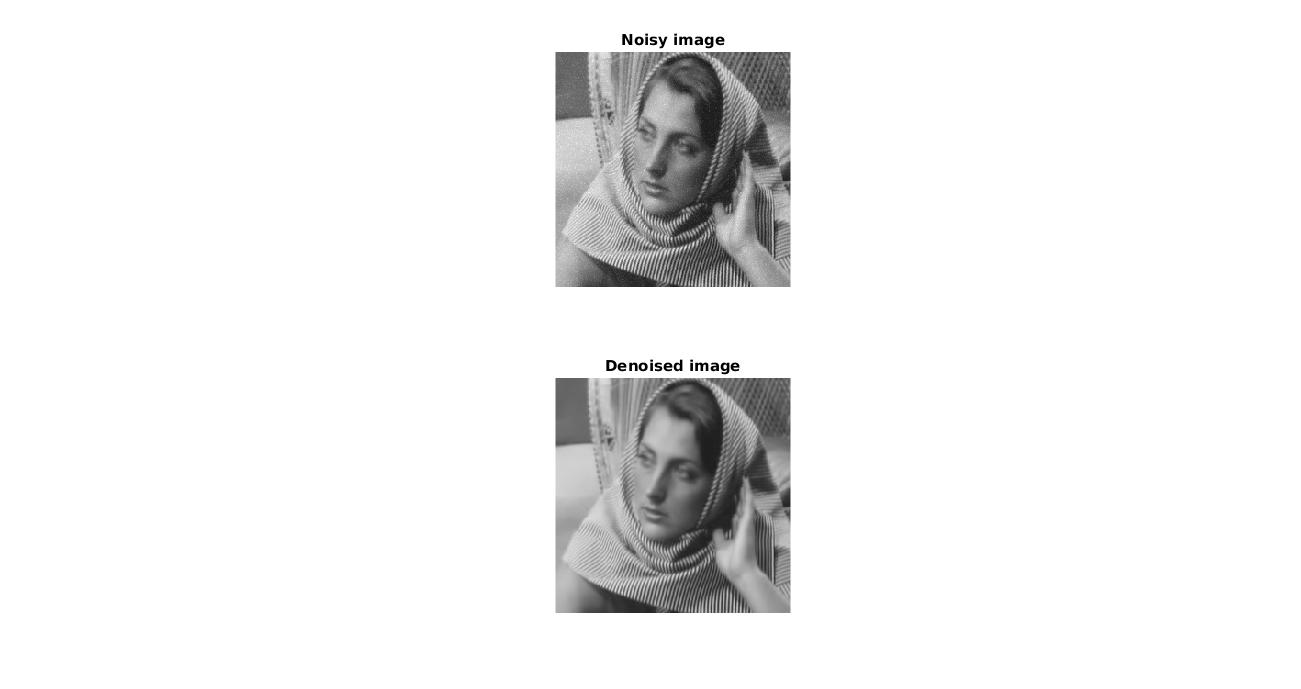
\includegraphics[scale=0.5]{q1a.jpg}
	\caption{Question 1a results}
	\label{Fig :1a}
\end{figure}

% \begin{figure}[h]
%   % \centering
%   \begin{subfigure}[t]{0.32\textwidth}
%     \centering
%     \includegraphics[scale=0.5]{images/original_image_barbara}
%     \caption{Original Image Barbara}
%     \label{Fig :1a}
%   \end{subfigure}
%   ~
%   \begin{subfigure}[t]{0.32\textwidth}
%     \centering
%     \includegraphics[scale=0.5]{images/noisy_image_barbara}
%     \caption{Noisy Image Barbara}
%     \label{Fig :1b}
%   \end{subfigure}
%   ~
%   \begin{subfigure}[t]{0.32\textwidth}
%     \centering
%     \includegraphics[scale=0.5]{images/denoised_image_barbara}
%     \caption{Denoised Image Barbara}
%     \label{Fig: 1c}
%   \end{subfigure}

%   \caption{Figures for Q1}
% \end{figure}

\subsection*{A1.2}

The code for this is question1b.m. The output is a little dark. Despite trying for different values of lambda and alpha the issue doesn't seem to get resolved.

Parameters chosen:
$$\lambda = 20$$
$$\alpha = 1.01*\text{max}(\text{eig}(A'*A))$$

\begin{figure}[h]
	\centering
	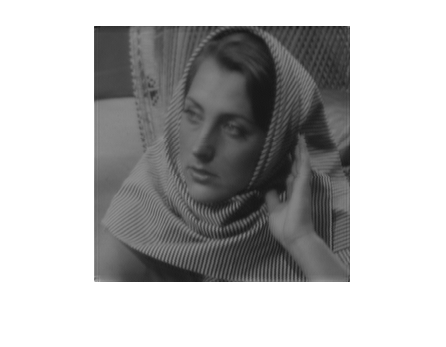
\includegraphics{html/mainScript_02.png}
	\caption{Question 1b result}
	\label{Fig :1b}
\end{figure}

% \begin{figure}[h]
%   \begin{subfigure}[t]{0.5\textwidth}
%     \centering
%     \includegraphics[scale=0.5]{images/original_image_barbara}
%     \caption{Original Image Barbara}
%     \label{Fig :1a}
%   \end{subfigure}
%   ~
%   \begin{subfigure}[t]{0.5\textwidth}
%     \centering
%     \includegraphics[scale=0.5]{images/phi_reconstructed_barbara}
%     \caption{Reconstructed Image Barbara}
%     \label{Fig :1b}
%   \end{subfigure}
%   \caption{Figures for Q2}
% \end{figure}

\subsection*{A1.3}
% In the folder q1, run the file deblur.m to get the deblurred image.

The code for this is question1c.m. The code takes a parameter of the magnitude of the noise relative to the magnitude of the signal expressed in percentage.


\section*{Q2}
\subsection*{A2}

There are several codes for this part. Firstly plot\_dct\_coefficient.m takes in paramters $(u,v)$ and plots distribution of the DCT coefficients of F$(u,v)$ . Another code is plot\_patch\_variances.m which plots the variances of the plots and hence was used to estimate the parameter $b$ of the uniform distribution. The function eval\_integral.m performs numerical integration of the given function. Also the given integral has a closed from expression in the terms of error function of the gaussian which we solved for and checked with our numerical intergrator and MATLAB's in built function and it exactly matches. The function obtained is:

$$ p(x) =  \frac{2}{\sqrt{2 \pi b}} e^{-\frac{x^2}{2b}} - \frac{x}{b} \text{erfc}\big(\frac{x}{\sqrt{2b}}\big)\text{sgn}(x) $$ 

This equation can be obtained using the following steps. Consider,

$$ I = \int_0^z \text{exp} \bigg(-\frac{1}{y^2} \bigg) dy \ \ ; z > 0 $$ 
 
By a change of variables it becomes,  $ I = \int_{1/z}^{\infty} \frac{e^{-x^2}}{x^2} dx $. This can be solved using considering,

$$ I(a) = \int_{1/z}^{\infty} \frac{e^{-ax^2}}{x^2} dx  \implies \frac{\partial}{\partial a}I(a) =  -\int_{1/z}^{\infty} e^{-ax^2} dx
$$

which can be expressed in terms of $\text{erf}$ function which is a well known function and integrating the obtained expression back wrt a, from $1$ to $\infty$, we get the required integral $ I = z\text{exp}\bigg(- \frac{1}{z^2}\bigg) - \sqrt{\pi} \text{erfc}\bigg(\frac{1}{z}\bigg) $ . This is for a positive value of $z$. The expression for negative $z$ can be obtained similarly by taking care at certain steps. Also, the final proabability distribution is actually given by the integral 

$$ p(F(u,v)) = \sqrt{\frac{2}{\pi}}.\frac{1}{b}. \int_0^{\sqrt{b}} \text{exp} \bigg(- \frac{|F(u,v)|^2}{2x^2} \bigg) dx $$

\section*{Q3}
\subsection*{A3.1}

The main idea behind this is that a convolution kernel can be described using a circulant matrix. Each of the kernel which represents a derivative can be converted into a matrix and the convolution of that kernel with an image can be equivalently written as the product of that matrix with the vectorised version of that image. From equation (6) we note that, there are 4 terms to be considered.
The first term of those is : $\rho(f_{ik}.I_1)$. The image $I_1$  is vectorised and written as $v$ and using the idea described above we can write $f_{ik}$ as a matrix. Hence this term can be written as $\rho(A_1v)$. Similarly, we can deal with the other similar looking terms and combine all the matrices to give us something of the form $ (\sum_k A_k)v $ . This is for a single, specific filter. This term $ (\sum_k A_k) $ is written as a single term $ A_{j\rightarrow} $ giving us the required matrix. \\

The summation also consists of terms with the image $I$ which is known to us. Thus the convolution can be similarly expressed for this using a matrix multiplication with the vectorised version of the image $I$. Even for $I$ we have the convolutions expressed as matrices $A_k$. When the image $I$ is multiplied with each of these we get a constant vector $b_k$ and all these vectors from the different terms of the summation from equation (6) can be combined and summed to give a constant vector which we call $b$ .  Note that we get a $b$ for each filter and then to get the final value we need to sum over all the filters. \\ 

We need to note here that all the terms in the images are not involved in the third and fourth term and thus we need to take care of that fact while forming the matrices. \\

The point the is we still havent considered the $\rho(.) $ terms but this would affect the way we are constructing this system because of linearity of the system. This explains how we would go about constructing the matrices and vectors. \\



\subsection*{A3.2}
In equation (6), the last two terms are representative of the likelihood and the first two terms are denote the prior. \\
To put things more explicitly, the likelihood terms are, 
$$\lambda \sum_{i \in S_1,k} \rho(f_{i,k}\cdot I - f_{i,k}\cdot I_1)$$
$$\lambda \sum_{i \in S_2,k} \rho(f_{i,k}\cdot I_1)$$
and on the other hand, the prior terms are,
$$\sum_{i,k} \rho (f_{i,k}\cdot I_1)$$
$$\sum_{i,k} \rho(f_{i,k} \cdot I_1 - f_{i,k} \cdot I)$$ \\

The prior used in this paper is the mixed Laplacian model descibed as, 
$$Pr(I) \approx \prod_{i,k}Pr(f_{i,k} \cdot I)$$


The likelihood used in this paper is that the gradient of $I_1$ at all locations $S_1$ agree with the gradients of the input image $I$
and similarly gradient of $I_2$ at all locations $S_2$ agree with the gradients of the input image $I$. That is,\\
At all points $S_1$:
$$\nabla I_1 = \nabla I$$
At all points $S_2$
$$\nabla I_2 = \nabla I$$


\subsection*{A3.3}
The third term in the summation is given by $\lambda \sum_{i \in S_1,k} \rho(f_{i,k}\cdot I - f_{i,k}\cdot I_1)$. This is equivalent to $\lambda \sum_{i \in S_1,k} \rho(f_{i,k}\cdot I_2)$. \\

This model is based on the fact that the gradients the points in $S_1$ and $S_2$ will be the same as the $I_1$ and $I_2$ respectively when compared to the image. This inherently assumes that the gradients in the images $I_1$ and $I_2$ will not coincide and given that these are natural images this is possible with a high probability making the assumption valid. This directly implies the terms in $I_2$ corresponding to the points in $S_1$ would be very sparse and correspondingly with $I_1$ and $S_2$. In the prior model, we have assumed a sub-laplacian model on the basis of statistics of natural images. This is the case when the gradients of $I$ and  $I_1$ are very similar and hence dense. In this the likelihood terms they are even sparser and would follow a GGD with a smaller shape parameter. Hence it is definitely incorrect to have a gaussian estimate instead of a laplacian or a sub-laplacian model. Thus to continue using the current model is a much better approximation than having a gaussian likelihood. This arguments holds for both the third and the fourth terms in the summation as the argument of sparsity hold equally well for both of them. \\ \\


Note: Images of some of the questions are in the html folder if they are not in the report here.



\end{document}

